\documentclass[11pt,letterpaper]{article}
\usepackage[lmargin=1in,rmargin=1in,tmargin=1in,bmargin=1in]{geometry}
\usepackage{../style/homework}
\usepackage{../style/commands}
\setbool{quotetype}{true} % True: Side; False: Under
\setbool{hideans}{false} % Student: True; Instructor: False

% -------------------
% Content
% -------------------
\begin{document}

\homework{6: Due 03/09}{Always remember that you are absolutely unique---just like everyone else.}{Margaret Mead}

% Problem 1
\problem{10} Given the feasible region shown below, find the minimum value of $f(x_1, x_2)= 8x_1 + 6x_2$. Does the function $f(x_1, x_2)$ have a maximum value on the same feasible set? Explain. 
	\[
	\fbox{
	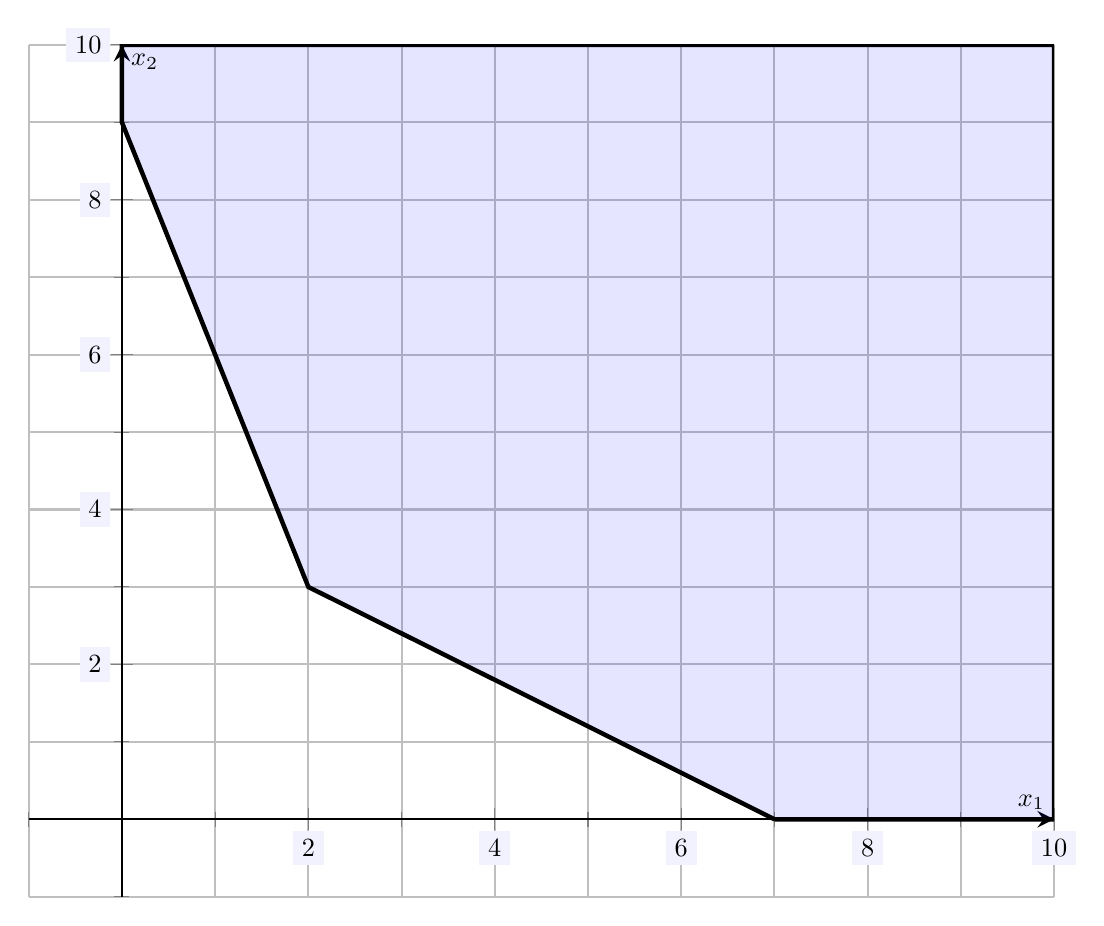
\begin{tikzpicture}[scale=1.9,every node/.style={scale=0.5}]
	\begin{axis}[
	grid=both,
	axis lines=middle,
	ticklabel style={fill=blue!5!white},
	xmin= -1, xmax=10,
	ymin= -1, ymax=10,
	xtick={0,2,4,6,8,10},
	ytick={0,2,4,6,8,10},
	minor tick = {-1,0,1,...,10},
	xlabel=\(x_1\),ylabel=\(x_2\),
	]
	\draw[line width=0.01cm,fill= blue,opacity=0.1] (7,0) -- (2,3) -- (0,9) -- (0,10) -- (10,10) -- (10,0) -- (7,0);
	\draw[line width=0.03cm] (7,0) -- (2,3) -- (0,9) -- (0,10) -- (10,10) -- (10,0) -- (7,0);
	\end{axis}
	\end{tikzpicture}
	}
	\] \pspace

\sol Because the feasible region is not bounded, the Fundamental Theorem of Linear Programming does not apply. Therefore, $f(x_1, x_2)$ does not necessarily have a maximum or minimum value on this feasible set. Observe that $f(x_1, x_2)$ is increasing in $x_1$ and $x_2$. Because $x_1$ and $x_2$ can be made arbitrarily large, $f(x_1, x_2)$ can be made arbitrarily large. Therefore, $f(x_1, x_2)$ has no maximum value on the feasible set. Vice versa, to minimize $f(x_1, x_2)$, we need to choose $x_1$ and $x_2$ as small as possible. Therefore, the minimum value for $f(x_1, x_2)$ on this feasible set should occur at a corner point. The corner points for this feasible set are $(0, 9)$, $(2, 3)$, and $(7, 0)$. We evaluate $f(x_1, x_2)$ at these corner points:
	\begin{table}[!ht]
	\centering
	\begin{tabular}{l | l}
	Corner Points & $f(x_1, x_2)$ \\ \hline
	$(0, 9)$ & $f(0, 9)= 8(0) + 6(9)= 54$ \\
	$(2, 3)$ & $f(2, 3)= 8(2) + 6(3)= 34$ \\
	$(7, 0)$ & $f(7, 0)= 8(7) + 6(0)= 56$
	\end{tabular}
	\end{table} \par
Therefore, as one can verify, the minimum value is $34$ and occurs at $(2, 3)$. 



\newpage


% Problem 2
\problem{10} Consider the minimization problem given below. As accurately as possible, sketch the feasible region given by the minimization problem. Is this minimization problem in standard form? Explain. Is there a guaranteed solution to this minimization problem? Explain. 
	\[
	\begin{aligned}
	\text{min } z= -3x_1 &+ 8x_2 \\
	x_1 - x_2&\geq -5 \\
	7x_1 + x_2&\leq 35 \\
	x_1, x_2&\geq 0
	\end{aligned}
	\]
	\[
	\fbox{
	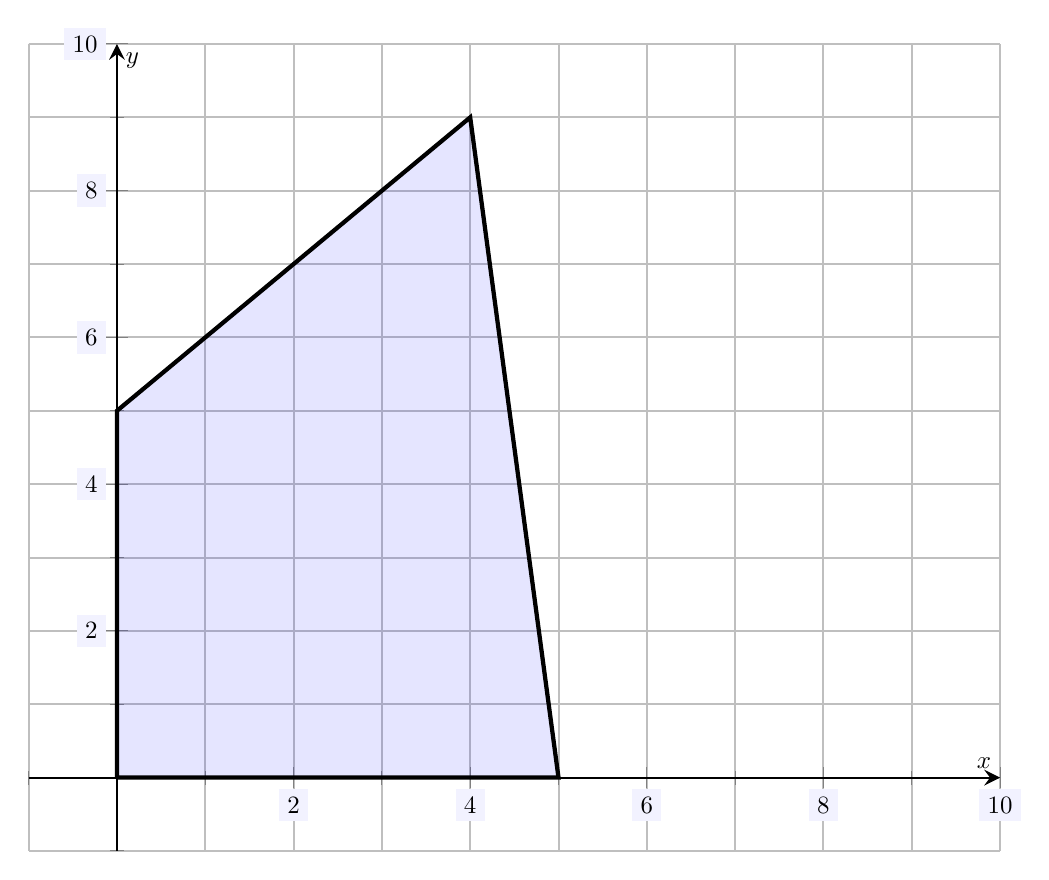
\begin{tikzpicture}[scale=1.8,every node/.style={scale=0.5}]
	\begin{axis}[
	grid=both,
	axis lines=middle,
	ticklabel style={fill=blue!5!white},
	xmin= -1, xmax=10,
	ymin= -1, ymax=10,
	xtick={0,2,4,6,8,10},
	ytick={0,2,4,6,8,10},
	minor tick = {-1,0,1,...,10},
	xlabel=\(x\),ylabel=\(y\),
	]
	\draw[line width=0.01cm,fill= blue,opacity=0.1] (0,0) -- (0,5) -- (4,9) -- (5,0) -- (0,0);
	\draw[line width=0.03cm] (0,0) -- (0,5) -- (4,9) -- (5,0) -- (0,0);
	\end{axis}
	\end{tikzpicture}
	}
	\] \pspace

\sol Because $x_1, x_2 \geq 0$, we only need to consider the region in Quadrant~I. Solving for $x_2$ in the first two inequalities, we find $x_2 \leq x_1 + 5$ and $x_2 \leq -7x_1 + 35$. Therefore, we shade below the line $x_2= x_1 + 5$ and below the line $x_2= -7x_1 + 35$. The line $x_2= x_1 + 5$ has $y$-intercept $(0, 5)$ and the line $x_2= -7x_1 = 35$ has $x$-intercept $(5, 0)$. The lines $x_2= x_1 + 5$ and $x_2= -7x_1 + 35$ intersect at the point $(4, 9)$. This gives the region shaded above. \pspace

The linear programming problem given is in standard form if (because it is a minimization) the function $z= -3x_1 + 8x_2$ is linear (it is), the decision variables are nonnegative (they are), and each inequality is of the form $\cdots \geq \text{non-neg \#}$---which is not the case for the first and second inequalities. Therefore, this problem is not in standard form. \pspace

Because this region is nonempty and bounded, the Fundamental Theorem of Linear Programming applies. Therefore, $z= -3x_1 + 8x_2$ has a maximum and minimum value and they occur at a corner point of the feasible region. 



\newpage



% Problem 3
\problem{10} Assume the following is an `initial simplex tableau associated to a standard minimization problem.' Write down the function being minimized and the corresponding system of constraints. Explain how the function and corresponding system of constraints changes if the problem were a standard maximization problem.
	\begin{table}[!ht]
	\centering
	\begin{tabular}{rrrrrr|r}
	$4$ & $-2$ & $6$ & $5$ & $1$ & $0$ & $125$ \\
	$3$ & $0$ & $-3$ & $5$ & $0$ & $1$ & $340$ \\ \hline
	$-1$ & $3$ & $-2$ & $-6$ & $0$ & $0$ & $0$ 
	\end{tabular}
	\end{table} \pspace

\sol The last row corresponds to the function while the other rows correspond to inequalities. Therefore, we have two inequalities and hence we have two slack variables. The last row would correspond to the function and we would have $z - x_1 + 3x_2 - 2x_3 - 6x_4= 0$. Therefore, the function being minimized is $z= x_1 - 3x_2 + 2x_3 + 6x_4$. Then the minimization problem is\dots
	\[
	\begin{aligned}
	\text{min } z= x_1 - 3x_2 + 2x_3 &+ 6x_4 \\
	4x_1 - 2x_2 + 6x_3 + 5x_4&\geq 125 \\
	3x_1 - 3x_3 + 5x_4&\geq 340 \\
	x_1, x_2, x_3, x_4&\geq 0
	\end{aligned}
	\]



\newpage



% Problem 4
\problem{10} Find the dual problem to\dots
	\[
	\begin{aligned}
	\text{min } w= 6x_1 - 7x_2 &+ 9x_3 \\
	x_1 + 7x_2 - x_3&\geq 10 \\
	2x_1 - 4x_3&\geq 5 \\
	x_1 + 5x_2 + 4x_3&\geq 10 \\
	x_1, x_2, x_3&\geq 0 
	\end{aligned}
	\] \pspace

\sol First, observe that the given minimization problem is in standard form. Now we find the matrix associated to the given linear programming problem:
	\[
	\begin{pmatrix}
	1 & 7 & -1 & 10 \\
	2 & 0 & -4 & 5 \\
	1 & 5 & 4 & 10 \\
	6 & -7 & 9 & 0 
	\end{pmatrix}
	\]
Now we compute the transpose of this matrix:
	\[
	\begin{pmatrix}
	1 & 2 & 1 & 6 \\
	7 & 0 & 5 & -7 \\
	-1 & -4 & 4 & 9 \\
	10 & 5 & 10 & 0 
	\end{pmatrix}
	\]
This matrix then corresponds to the following maximization problem, i.e. the dual problem:
	\[
	\begin{aligned}
	\text{max } w= 10y_1 + 5y_2 &+ 10y_3 \\
	y_1 + 2y_2 + y_3&\leq 6 \\
	7y_1 + 5y_3&\leq -7 \\
	-y_1 - 4y_2 + 4y_3&\leq 9 \\
	y_1, y_2, y_3&\geq 0 
	\end{aligned}
	\]


\end{document}